\section{Exercise 3.2 - ModuleDouble}

For ModuleDouble, the application now includes two threads, one method and four events. We use dynamic sensitivity in this exercise to subscribe and wait for an event to trigger the method. Figure \ref{fig:moduledouble} shows the interaction between the threads A and B and method A.

\begin{figure}[h]
	\centering
	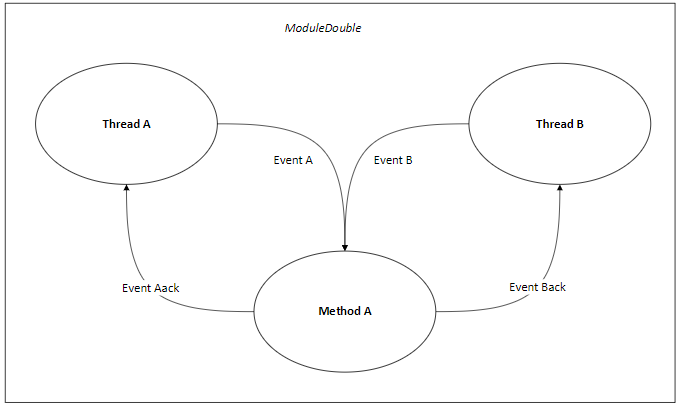
\includegraphics[width=1\linewidth]{ModuleDouble.png}
	\caption{Architecture of ModuleDouble with threads, methods and events.}
	\label{fig:moduledouble}
\end{figure}

The application file contains the main.cpp which instantiates ModuleDouble and starts the simulation as shown in listing \ref{lst:moduledoublemain}.

\begin{lstlisting}[style=customc++, caption=Application file for ModuleDouble,
label={lst:moduledoublemain}]
#include "ModuleDouble.h"
int sc_main(int argc, char* argv[]) {
	moduleDouble my_module("moduleDouble");
	sc_start(2000,SC_MS);
return 0;
}
\end{lstlisting}

The logic is implemented in the ModuleDouble.h file. Firstly, we define the four events that are used to trigger the threads and methods as shown in the architecture. We then introduce a boolean event\_tracker variable to enable the method A to alternate between waiting on event A and B. The two threads A and B notifies event A and B respectively and waits for an acknowledgment from the method by calling the \textit{wait()} method. This suspends the thread and waits for the sensitive list event to occur (event Aack and Back respectively). The method alternates between the two events, prints the current time and which event it has received before notifying the acknowledge event and waits for the opposite thread than the one being acknowledged to invoke it again using the \textit{next\_trigger()} method. The code for ModuleDouble.h is shown in listing \ref{lst:moduledoubleheader}. Note that the \textit{dont\_initialize()} method in the constructor prohibits the threads from being executed before the event occur.

\begin{lstlisting}[style=customc++, caption=Implementation of ModuleDouble,
label={lst:moduledoubleheader}]
SC_MODULE(moduleDouble){

sc_event event_a, event_b, event_a_ack, event_b_ack;
bool event_tracker;

void my_threadA(void) {
	while(true) {
		wait(3,SC_MS);
		event_a.notify();
		wait(3,SC_MS,event_a_ack);
	}
}
void my_threadB(void) {
	while(true) {
		wait(2,SC_MS);
		event_b.notify();
		wait(2,SC_MS,event_b_ack);
	}
}
void my_methodA(void){
	if(event_tracker) {
		std::cout << "Timestamp: " << sc_time_stamp() << "
		- event: A" <<  std::endl;
		event_a_ack.notify();
		event_tracker = false;
		// When the method is called next time it must be by event_b
		next_trigger(event_b);
	} else {
		std::cout << "Timestamp: " << sc_time_stamp() << "
		- event: B" <<  std::endl;
		event_b_ack.notify();
		event_tracker = true;
		// When the method is called next time it must be by event_a
		next_trigger(event_a);
	}
}
SC_CTOR (moduleDouble) {
	SC_THREAD(my_threadA)
	sensitive << event_a_ack;
	SC_THREAD(my_threadB)
	sensitive << event_b_ack;
	SC_METHOD(my_methodA)
	sensitive << event_a << event_b;
	dont_initialize();
} };
\end{lstlisting}